\section{Project Documentation}
\subsection{Project Overview}
\noindent The purpose of this project is to implement a work flow of big data. The following digram shows loading new data into DynamoDB starts with S3. The new record is stored in S3 firstly. When it is imported to DynamoDB, we have to check whether the identifier for the device or person is new. If the unique identifiers are new, a new system identifier is generated based on a hash of the original device and student identifiers. The original device and student identifiers are loaded to Identity table. On the other hand, the original identifiers are replaced with the new system identifier, and the anonymized record is loaded into a DynamoDB data table. If the unique identifiers are not new, they are replaced with the system identifier already available in the Identity table, and the record is added to the data table.
\begin{figure}[H]
	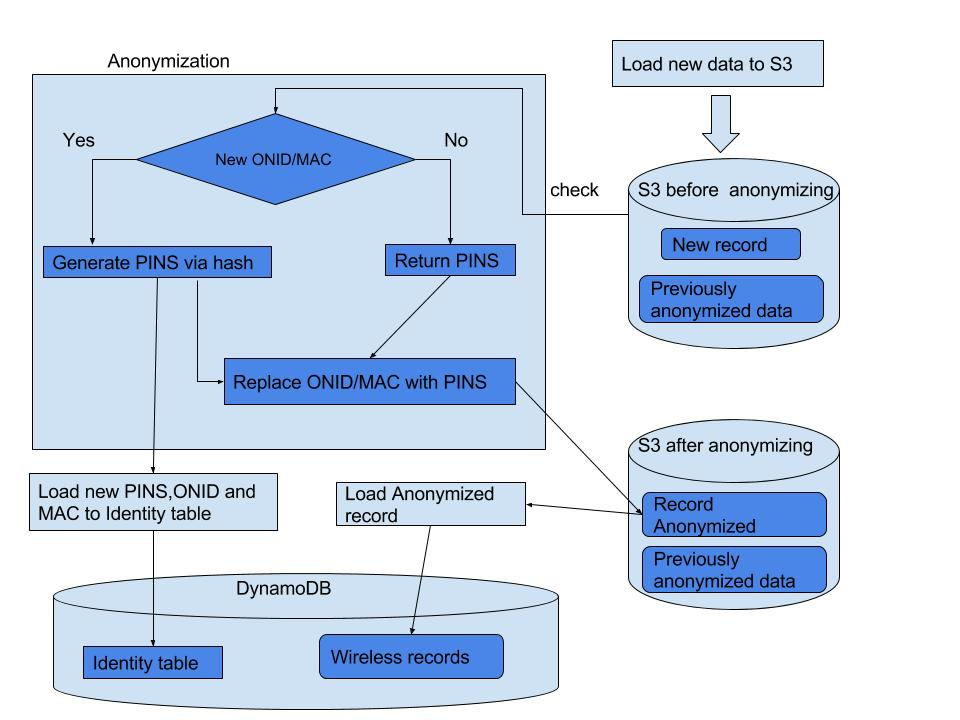
\includegraphics[width=17cm, height=12cm]{Pictures/workflow.jpg}
    \centering
    \caption{\label{fig:2}The workflow of importing new record}
\end{figure}

\noindent The workflow of the visualization starts from S3. After the DynamoDB table results have been stored back into S3, the data will be stored as CSV files in S3. These CSV files are important to the QuickSight because it requires the CSV files to generate the data set on the QuickSight console. After the data set have been created on the QuickSight console, the visualization will be easily generated. The figure \ref{fig:3} is the workflow of creating visualization on QuickSight.  

\begin{figure}[H]
	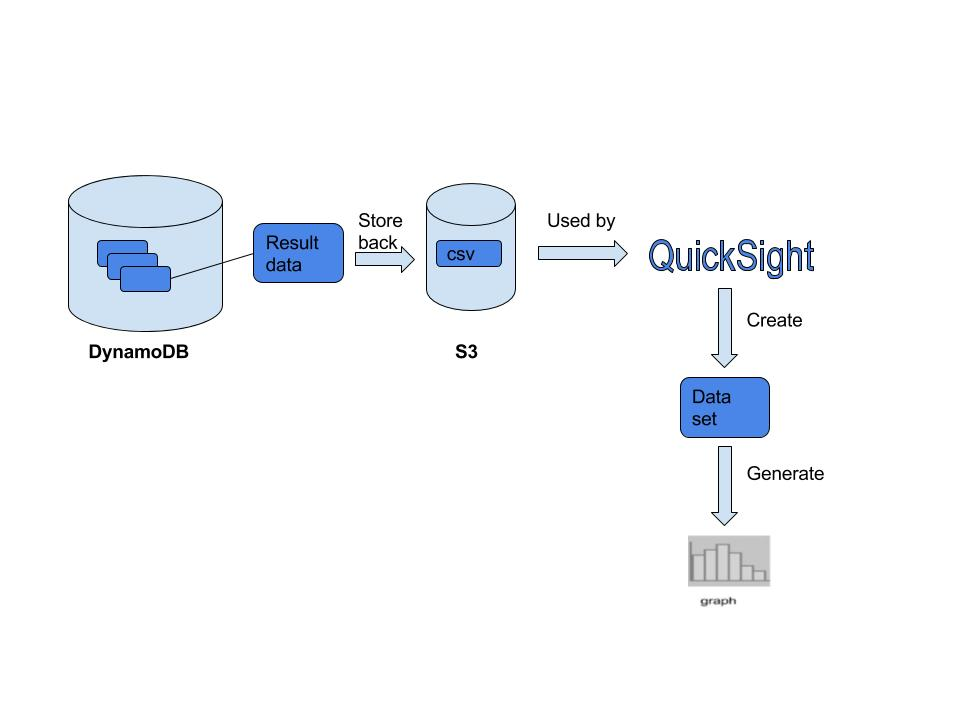
\includegraphics[width=17cm, height=10cm]{Pictures/QuickSight_workflow.jpg}
    \centering
    \caption{\label{fig:3}The workflow of creating visualization on QuickSight}
\end{figure}


\subsection{Operating instructions}
The project is working on the Amazon Web services, so it requires you must have a AWS account and this account has permission to access our project.\\

\noindent Load data from S3 into DynamoDB:
\begin{itemize}
	\item Connecting into the EC2 instance, run the python file \texttt{create.py} for creating table
    \item After creating tables, run the \texttt{import.py} for loading data login in the DynamoDB
    \item The command you need to type is \texttt{python import.py [input bucket name] [input file name] [output bucket name]}. The input bucket is the path of input file, and output bucket is the path of anoymized record.
    \item Check the result on the console Stop the EC2 instance on EC2 console
\end{itemize}

\noindent Save the result back to the S3:
\begin{itemize}
	\item Anonymized record have been created after run the import.py 
    \item This record is stored in a certain bucket
\end{itemize}

\noindent Create visualization on the QuickSight
\begin{itemize}
	\item Open the QuickSight console on AWS and Click New analysis button
    \item Choose New data set and click upload a file and choose the csv file which export from the "Records" table
    \item Using the data set and select the conlumn which need to evalaute
    \item Select the rows that need to evaluate and choose the visual types
    \item The visual will be created on right side    
\end{itemize}



